% Section content template for individual Educative lessons
% This file contains the actual content for a specific section
% Generated from Educative API section content

% Section: Evaluation of Quora’s Design
% Section ID: 5580185650331648
% Section Slug: evaluation-of-quoras-design
% Generated: 2025-12-07T22:56:08.176683

\subsection{Requirements compliance}\label{xesAI2MOJEYpW9qCoEyk3}
\\
We have used various techniques to fulfill our functional requirements. However, we need to determine if we have fulfilled the non-functional requirements. We 'll highlight some of the mechanisms we have utilized to address the non-functional requirements:

\begin{itemize}
\item
\protect\phantomsection\label{I_N0H_7MNOCGBYDWsONVZ}
\textbf{Scalability:} Our system is highly scalable for several reasons. The updated design uses powerful and homogeneous service hosts(Quora now uses Amazon EC2 instances with 32 cores, a shared 20 MB cache, and high network throughput.). Quora uses powerful machines because service hosts use an in-memory cache, some level of queueing, maintain manager, worker, and routing library. The horizontal scaling of these service hosts is convenient because they are homogeneous.\\
On the database end, our design shards the MySQL databases vertically, which avoids issues in scalability because of overloaded MySQL servers. To reduce complex \texttt{join} queries, tables anticipating \texttt{join} operations are placed in the same shard or partition.
\end{itemize}
\begin{quote}
\textbf{Note:} As mentioned earlier, vertical sharding may not be enough because each shard can grow large horizontally. For large MySQL tables, writing becomes a bottleneck. Therefore, our design may have to adhere to horizontal sharding, a well-known practice in database scaling.
\end{quote}
\begin{itemize}
\item
\protect\phantomsection\label{hqkAXUZkWQVCFVrYp4M7p}
\textbf{Consistency:} Due to the variety of functionalities offered by Quora, different consistency schemes may be selected for different types of data. For example, certain critical data like questions and answers should be stored synchronously. In this case, performance can take a hit because users don't expect instantaneous responses to their questions. It means that a user may get a reply in five minutes, one hour, one day, or no response at all, depending on the user's question and the availability of would-be respondents.\\
Other data like view counts may not necessarily be stored synchronously because it is not a goal of the Quora service to ensure that all users see the same number of views as soon as the question is posted. For such cases, eventual consistency is favored for improved performance.
\end{itemize}
\begin{quote}
\textbf{Note:} In general, our design is equipped with strong techniques to reduce the user-perceived latency as a whole.
\end{quote}
\begin{itemize}
\item
\protect\phantomsection\label{m8f53CNddBrjeQeoj-NIR}
\textbf{Availability:} Some of the main ideas to improve availability include isolation between different components, keeping redundant instances, using CDN, using configuration services like ZooKeeper, and load balancers to hide failures from users.
\end{itemize}

Decoupling services help to maintain, upgrade, and recover during failures of individual service or hosts. If services are collocated on the same node or host, a failed node results in the loss of multiple services at once.

Our design, however, lacks any disaster recovery management, which we'll explore in the next section.

\begin{itemize}
\item
\protect\phantomsection\label{jZgPCoXdzVyZI9kS9XG8T}
\textbf{Performance:} This design has a strong performance because we have employed the right technology for the right feature. For example, we have used several datastores for different reasons. On top of that, we used different distributed caches depending upon the use case and access frequency. Also, we employed Kafka to queue similar tasks and assign them to cron jobs that otherwise take a long time if executed via API calls.
\end{itemize}

\begin{enumerate}
\def\labelenumi{\arabic{enumi}.}
\item
Quora has developed a custom in-memory caching system called Pycache that can store tens of GBs of cache in a local machine.
\\
The Pycache API contains simple but effective functions like \texttt{pycache.get(key)}, pycache.set(key,\ value), \texttt{pycache.delete(key)}, \texttt{pycache.iteritems()}, and \texttt{pycache.update()}.
\\
Both the \texttt{set} and \texttt{delete} functions have variants to set and delete multiple entries at once.
\item
Quora has developed an open-sourced tool called \textbf{Asynq} that simplifies batching of cache requests to Memcached. So, developers can write code faster---and the latency of a round trip to the caching service is reduced.
\end{enumerate}

\textbf{Non-functional Requirements Compliance}

\begin{table}[htbp]
\centering
\small
\adjustbox{max width=\textwidth}{
\begin{tabular}{|p{0.157\textwidth}|p{0.793\textwidth}|}
\hline
\textbf{Requirements} & \textbf{Techniques} \\
\hline
\hline
Scalability & \begin{itemize} \tightlist \item Based on AWS, which supports automatic scaling. \item Uses the same servers to reduce complexity in horizontal scalability \item sharding of MySQL database. \item Employs various data stores for different purposes. \item Asynq can enable developers to code quickly by batching cache requests, \item separate compute, and feature extraction modules. Therefore, a generic feature extraction facility allows scalability of different recommendation systems. \end{itemize} \\
\hline
Consistency & \begin{itemize} \tightlist \item Uses MySQL and synchronous replication within a data center for critical data. \item Offers eventual consistency for non-critical data like the view counter. \end{itemize} \\
\hline
Availability & \begin{itemize} \tightlist \item Use of different data stores prevents failure of multiple services at once by \item using database sharding and replicas. \item Uses CDN as a backup to serve static/dynamic data in case of failures. \item ZooKeeper enables service hosts to get updates about MySQL shards. \item Load balancers hide server failures from end users. \item AWS supports an availability above 99 percent. \item Thrift isolates services and therefore failures. \end{itemize} \\
\hline
Performance & \begin{itemize} \tightlist \item MyRocks has a much lower P99 latency. \item Uses the right programming language to deliver tasks quickly, such as C++ for the routing library. \item Uses `Multiget()`~ to retrieve multiple entries from Memcached at once. \item Eliminates network round trip time with Asynq. \item Kafka improves the performance of service hosts. \item Sharding improves QPS of MySQL. \item Custom, in-memory caching system reduces the latency of frequently accessed data. \end{itemize} \\
\hline
\end{tabular}
}
\caption{Non-functional Requirements Compliance}
\end{table}

\subsection{Disaster recovery}\label{Jk--_uoRMbOA--Qczw9He}
\\
Our proposed and detailed design does not cater to the situation of natural disasters(Disasters include large-scale floods, earthquakes, fires, and outages on multiple backbone Internet connections taking off a whole data center or multiple data centers.). While we have met other non-functional requirements, durability, fault-tolerance, and availability are incomplete without a disaster recovery management plan. This section will explore some mechanisms that provide resilience against disasters.
\\
The first and foremost approach of handling a disaster is frequent backups. The frequency of backups depends on the size of the data. Daily backups are suitable for our design because we can backup individual data stores and shards without any hassle. Of course, backups will be stored at remote destinations because natural disasters can wipe out the entire facility at a location.
\begin{quote}
\textbf{Note:} Taking regular backup at remote locations is not enough. Quick restoration of backed-up data in a timely manner completes a disaster recovery plan.
\end{quote}
\\
The following are important questions for designing a disaster recovery plan:

\begin{itemize}
\item
\protect\phantomsection\label{0LPeK2VGOnOM24Y5GBne4}
What data and systems are considered critical to recover from disasters?
\item
\protect\phantomsection\label{pld_eVQziXjKyjn4-eaa8}
How fast is the restoration from the backup facility?
\item
\protect\phantomsection\label{xKJA0suX8hMRDFqLMMi_D}
Can all systems be recovered through backups?
\item
\protect\phantomsection\label{z_-DwD0DvZ4xirkGVBaCA}
How can we deal with potential loss of data that we couldn't replicate before the disaster hit?
\end{itemize}
\\
The illustration below shows a simple architecture of how a disaster recovery scheme works:

\begin{figure}[htbp]
 \centering
 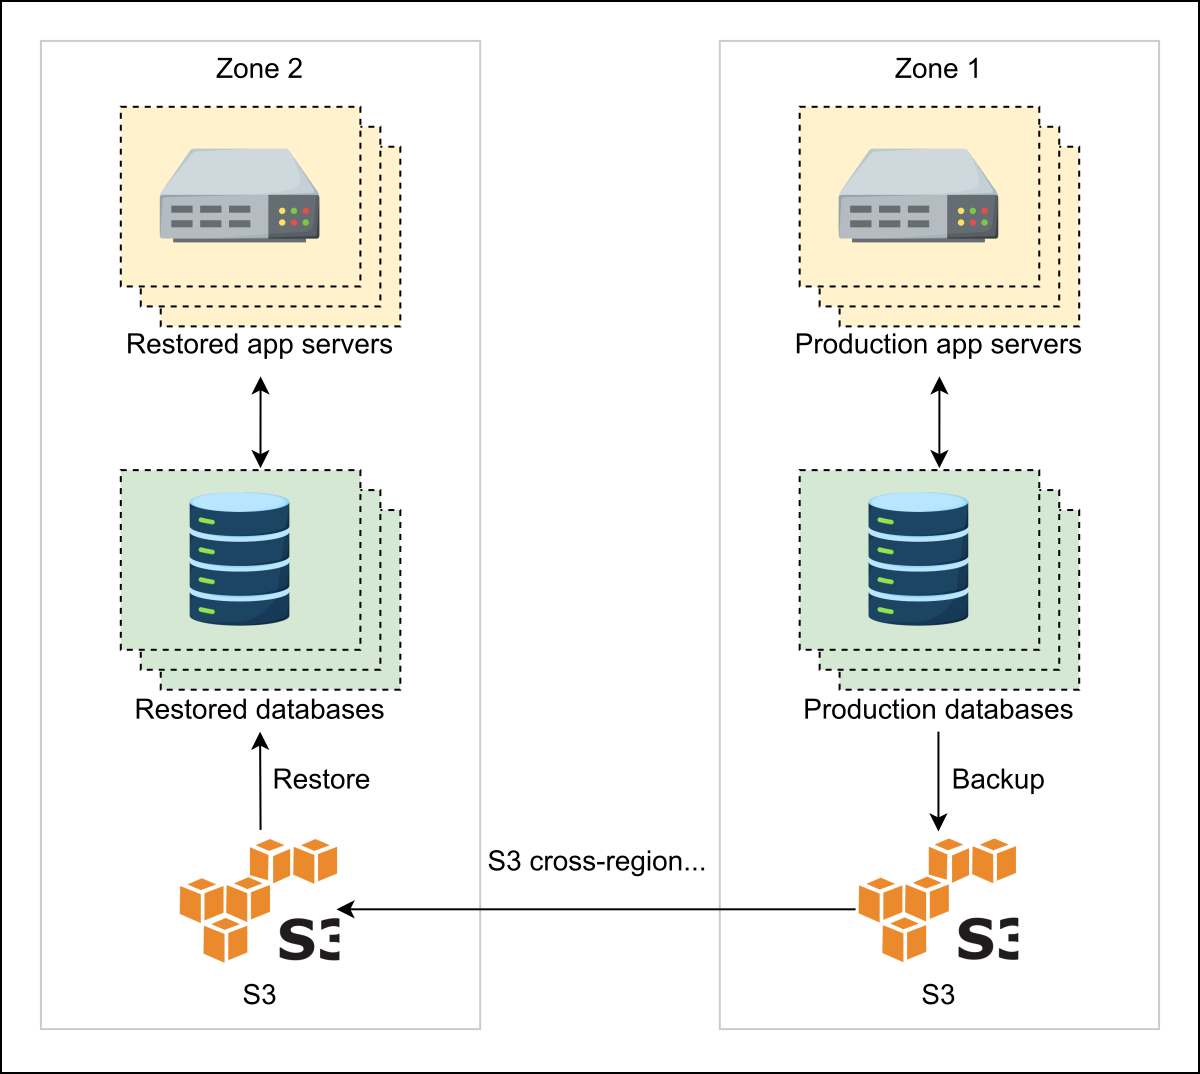
\includegraphics[width=0.5\textwidth]{Images/chapter_27/section_5580185650331648/5183834369163264.png}
 \caption{Disaster recovery management}
\end{figure}

The approach is fairly straightforward. The data, application servers, and configurations are backed up in the Amazon S3 storage service in the same zone. Zonal replication between S3 storage facilitates transfer to another zone. Later , the application and database servers can be restored from the S3 storage in another zone.
\\
The restoration strategy is simple and effective but it has a couple of drawbacks:

\begin{itemize}
\item
\protect\phantomsection\label{xYJoBdmIfy0cq5CLNvEjn}
We might lose some data that is not backed up since we take backups on a daily basis. However, this issue can be mitigated if we do synchronous replication across regions.
\item
\protect\phantomsection\label{Z38x8Oy_6uvgOL8HVze5X}
Restoration can take a long time (a few hours), and most databases do not serve queries while data is being recovered.
\end{itemize}
\begin{quote}
\textbf{Note:} In general, Amazon provides service with high reliability and availability. For instance, S3 service reports 99.999999999\% durability and 99.9\% availability over a year.
\end{quote}
\subsection{Conclusion}\label{dm2kXAxRbBkjgMdfq0MOE}
\\
Throughout this design, we learned how Quora is able to scale its services as the number of users increases. One interesting aspect of the design includes the vertical sharding of the MySQL database. Apart from that, the Quora design discusses a variety of techniques to meet the functional and non-functional requirements. However, our scope did not include the usage of techniques like natural language processing (NLP) to remove spelling mistakes in user's questions or typeahead services during the search.

\begin{quote}
\textbf{Quiz:}
\textbf{Question 1:} How can using different data stores for different types of data be beneficial in disaster recovery?
\textbf{Answer:} When we use different data stores, it means that we can recover various forms of data simultaneously instead of one large blob of data. Since we recover data stores with variable recovery times, the final recovery time equals the maximum recovery time among all data stores. However,

using many databases also means that administrators need to know the details of checkpointing or restoring them.
\end{quote}

% End of section content